%!TEX root = virtual-clusters.tex
%%% Local Variables:
%%% mode: latex
%%% TeX-master: t
%%% End:

\section{Cloudmesh Client} \label{S:cloudmesh}

The Cloudmesh Client toolkit \cite{www-cloudmesh} is a lightweight
client interface for accessing heterogeneous clouds, clusters, and
workstations right from the user's computer.  The client has its
origin in \cite{Laszewski2007,laszewski09,laszewski10}. With the
client a user can manage their own set of resources enabling management of a
personalized cyber infrastructure. It includes an API, a commandline
client, and a commandline shell.  Extensibility is provided via
convenient abstractions.  A local database allows caching of
information from remote resources.  This is an essential feature of
Cloudmesh as it allows users to preserve a view of the infrastructure
even in cases where it may not be reachable. Obviously, such a cache is
especially useful for large scientific workflows and services that
require the management of many tasks.  Administrators naturally need
such a cached view in order to identify faults and to effectively
preserve the view of resources that need to be accessed or have been
created in the past.

Furthermore, users can, via the provided abstractions, switch easily
between or utilize together virtual machines from OpenStack, Amazon,
Azure Clouds, and \Comet~virtual clusters \cite{comet14}. Hence a greater ability to
deal with faults or system failures can be achieved. Cloudmesh Client
can be installed on Linux, OSX, and Windows. Currently we support
backends to SLURM, SSH, OpenStack, Azure, and AWS. A Docker interface
is planned.\footnote{In the past we supported AWS and Azure which we
  are integrating back into the client and will be available at time
  of publication. Our main focus so far was the ability to add
  OpenStack in support of upcoming systems such as Jetstream and
  virtual clusters such as used in \Comet } Next we provide a short
overview of the main features of the Cloudmesh Client.

{\parindent 0pt \bf Client based.} Cloudmesh Client as the name
indicates is a client based toolkit that installs and runs on the
users or administrators computers. An optional prototype portal is
also available as an add on.

{\parindent 0pt \bf Layered Architecture.} Cloudmesh Client has a
layered architecture (Figure \ref{F:arch-layer}) that allows easy
development of new features. This also allows contribution by the
community while developing integrated and smaller sub components. A
resource abstraction layer allows the integration of a multitude of
resources spanning HPC, Containers, and Cloud resources. This layered
architecture is augmented with a number of components (Figure
\ref{F:arch-component}) that together build the overall and expandable
Cloudmesh Client architecture providing a rich feature set.

\begin{figure}[!h]
  %\centering   
    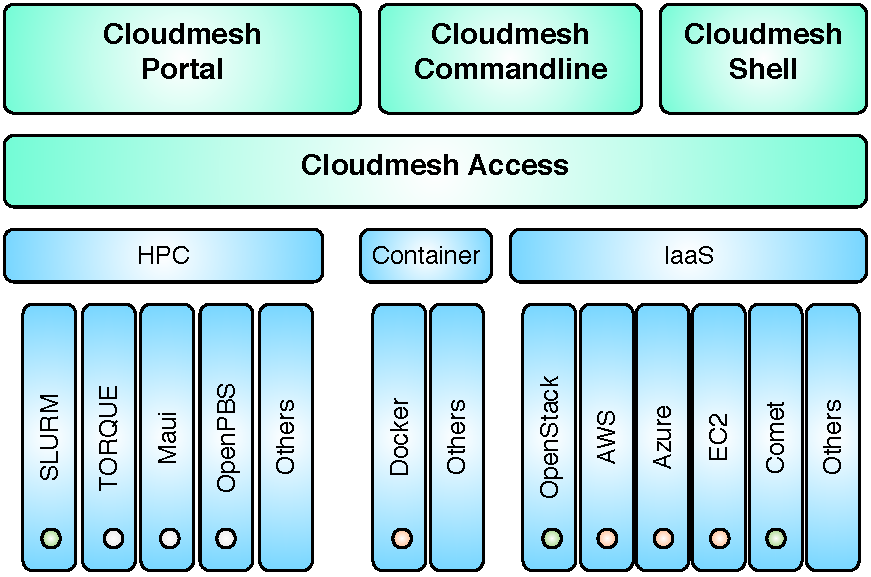
\includegraphics[width=1.0\columnwidth]{images/client/cloudmesh-arch-1.pdf}
    \caption{Cloudmesh layered architecture.}
    \label{F:arch-layer}
%\end{figure}
\bigskip
%\begin{figure}[!h]
  %\centering
    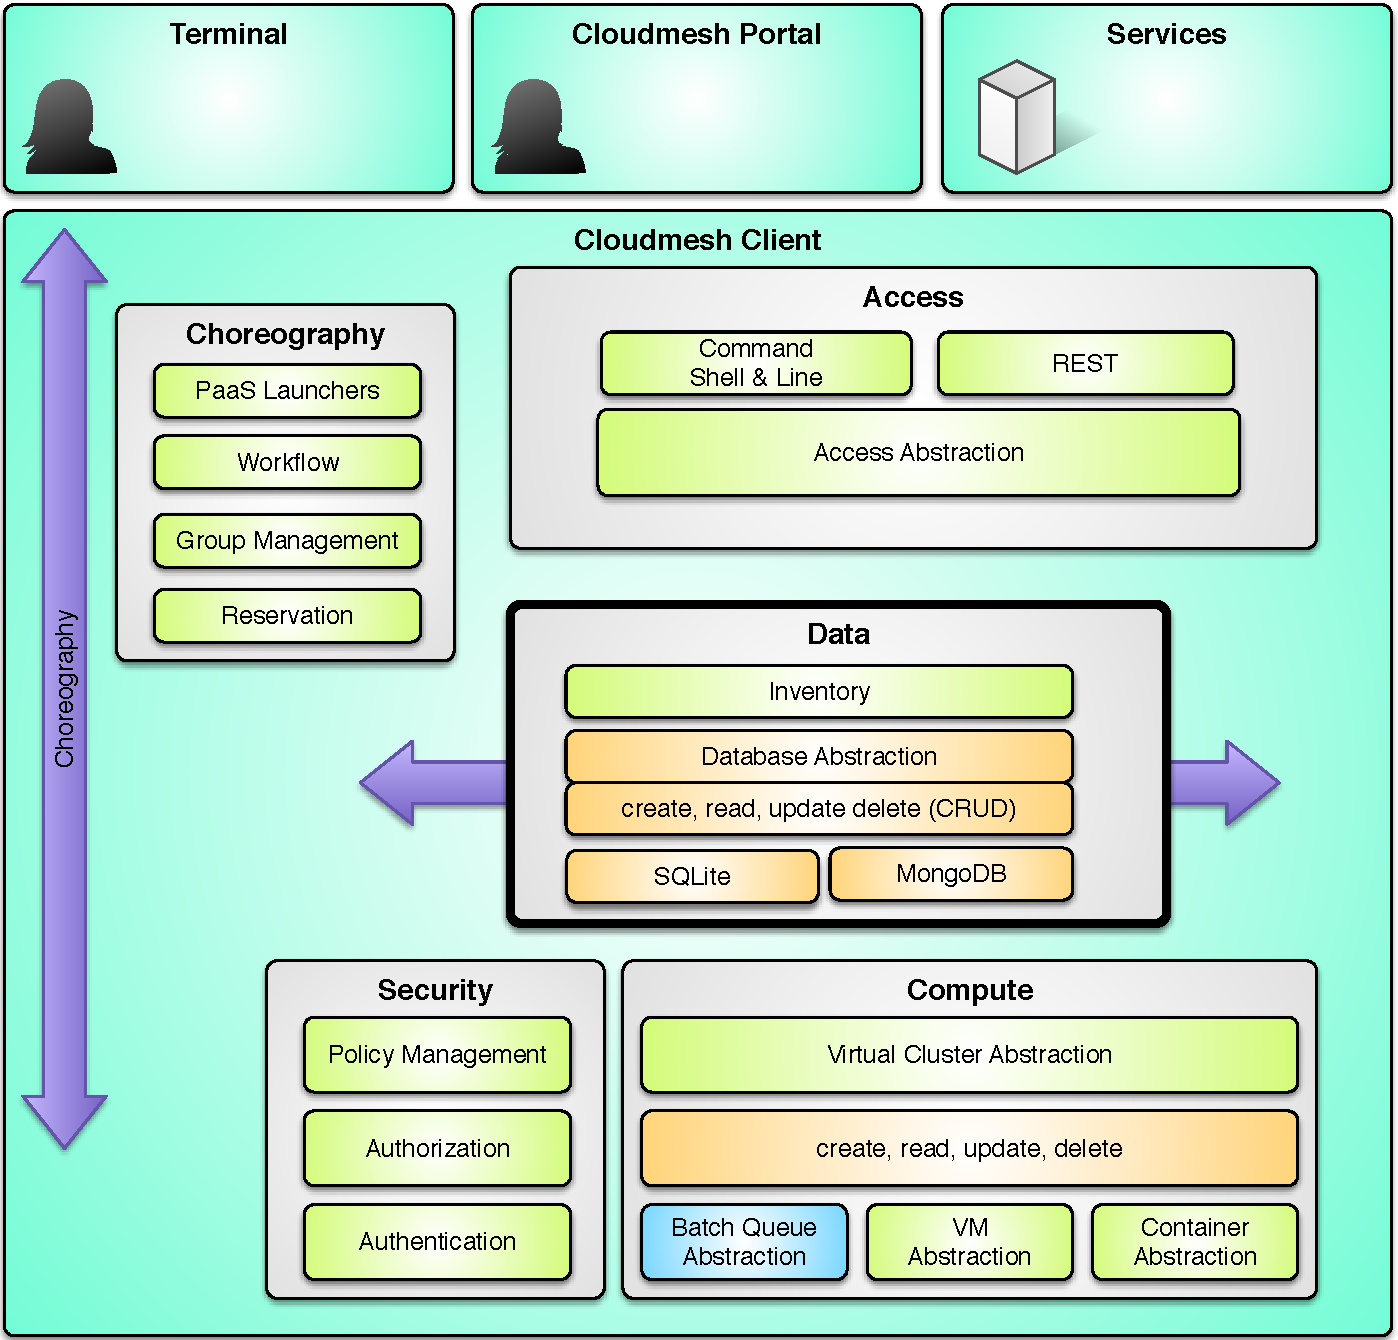
\includegraphics[width=1.0\columnwidth]{images/client/cloudmesh-arch-2.pdf}
    \caption{Cloudmesh component overview}
    \label{F:arch-component}
%\end{figure}

\bigskip

%\begin{figure}[htb]

{\tt cm comet cluster  ID}\newline -- Show the cluster details

{\tt cm comet start ID vm-ID-[0-3] --walltime=6h}\newline -- Boot 3 nodes for 6 hours

{\tt cm comet iso attach image.iso ID vm-ID-3}\newline -- Attach an iso image

{\tt cm comet power on ID vm-ID-0}\newline -- Power on node 0

{\tt cm comet console ID vm-ID-0}\newline
-- open the console for the node

\caption{Example Comet client commands}
\label{F:commands}
\end{figure}


\parindent 0pt { \bf State Caching.} Cloudmesh contains necessary state
about the resource and environment that a user may want to use.  The
information is managed in a database abstraction that would allow
storing the data in a variety of databases such as SQL and MongoDB. At
this time we have chosen SQLite to be the default database as it does
not require any additional setup and is universally available on all
operating systems without change. Previously we also provided a
MongoDB based backend system, but for the \Comet~client it is
beneficial to interact with the system without the need of additional
services.

{\parindent 0pt \bf Security Management.} For \Comet~users, it is
beneficial that access to the backend services are enabled with secure
credentials managed on the user's machine as well as with token based
service access.  This reflects best practice by many supercomputing
centers. Through abstractions integration with hosted security
services \cite{BasneyHW05} would also be possible.  However our
integration in clouds is naturally done outside such frameworks and
allows user to individually add their credentials for services such as
Azure, AWS, and other public clouds into the client easily. We have an
exploratory project in place that looks at the use of Yubikeys for
Cloudmesh Client and Cloudmesh Portal \cite{yubikey}. This will allow
an additional 2 factor authentication as part of accessing services
used by the users.  Hence, the Cloudmesh Client deals with the secured
connection and interaction by considering the appropriate interactions
with the different backends.  For the \Comet~virtualized cluster, it
handles the initial apikey retrieval, once a user is authenticated to
the nucleus service. It also handles all the subsequent calls in a
secured fashion by dealing with the messages signing, encryption and
decryption via utilizing proper libraries.

\parindent 0pt { \bf Command Shell and Command Line.} Cloudmesh contains a
command shell allowing scripts and interactive use. However we
designed the command shell in such a way that each command can also be
called from the command line reducing development and maintenance
efforts. Through the Cloudmesh database abstraction the state is
synchronized between different components.

\parindent 0pt { \bf Cloudmesh Client Portal.} Previously, we
distributed Cloudmesh with client, server, and a portal in one
package. This however turned out to be too complex to be installed for
some of our less technically skilled user communities. Thus we split up
the original Cloudmesh into multiple independent packages, such as the
{\em Cloudmesh Client} and the {\em Cloudmesh Portal}. The portal
provides currently a minimal feature set to manage virtual machines
and HPC jobs. It showcases how to integrate the client and the rest
services in more elaborated portal frameworks. We will expand upon the
existing features and make the portal more feature complete. Due to
our focus on the \Comet~community, the commandline client has an
increased development priority as it allows users to automatize
advanced {\em DevOps} workflows through scripting.

\parindent 0pt { \bf Cloudmesh Comet.} We are actively developing the
client interface for SDSC's \Comet~\cite{www-comet-user-manual}
supercomputer allowing near bare metal provisioning. The interface
reuses Cloudmesh components and technologies while interfacing with
the {\em Comet} Nucleus REST interface. Through this interplay the virtual
cluster administrators are enabled to utilize tools and services that
the they typically use to manage an on-premise bare metal cluster. As
part of this development we have developed an easy to use high level
command line interface specifically targeted to {\em Comet's\/} features. This
includes the following functionality:

\begin{itemize}
\item Configuring the nucleus service endpoint and the authentication
  tokens or keys.
\item Getting information and status of the users cluster(s), nodes,
  computesets, and other entities.
\item Power management of the cluster frontend node.
\item Request resource allocation to boot the users node(s); and release
  the resource upon completion.
\item Power management to shutoff, power on, reboot compute node(s)
  during the lifetime of the requested resource allocation.
\item Getting console access to the frontend node or a running compute
  node
\item System ISO image management. This includes listing available ISO
  images, upload new images, and attach/detach an ISO to/from one or
  more compute nodes.
\item Convenient management commands to, for example, renaming compute
  nodes either individually or in batch.
\end{itemize}

Some example commands are depicted in Figure \ref{F:commands}. The
manual page is shown in Figure \ref{F:man}.


%%% Local Variables:
%%% mode: latex
%%% TeX-master: t
%%% End:
\begin{figure}[!h]
\begin{small}
\begin{verbatim}
comet init
comet ll [CLUSTERID] [--format=FORMAT]
comet cluster [CLUSTERID][--format=FORMAT]
comet computeset [COMPUTESETID]
                 [--allocation=ALLOCATION]
                 [--cluster=CLUSTERID]
                 [--state=COMPUTESESTATE]
comet start CLUSTERID 
            [--count=NUMNODES]
            [COMPUTENODEIDS]
            [--allocation=ALLOCATION]
            [--walltime=WALLTIME]
comet terminate COMPUTESETID
comet power (on|off|reboot|reset|shutdown) 
            CLUSTERID [NODESPARAM]
comet console CLUSTERID [COMPUTENODEID]
comet iso list
comet iso upload [--isoname=ISONAME] PATHISOFILE
comet iso attach ISONAME CLUSTERID [COMPUTENODEIDS]
comet iso detach CLUSTERID [COMPUTENODEIDS]
comet node rename CLUSTERID OLDNAME NEWNAME

Options:
  --format=FORMAT         Format is either table, json, 
                          yaml, csv, rest [default: table]
  --count=NUMNODES        Number of nodes to be powered on. 
                          When this option is used, the 
                          Comet system will find a NUMNODES 
                          number of arbitrary nodes that
                          are available to boot as a 
                          computeset
  --allocation=ALLOCATION Alocation to charge 
  --walltime=WALLTIME     Walltime requested for node(s).
                          An integer followed by a unit 
                          (m,h,d,w, for minute, hour, day)
                          E.g., 3h, 2d
  --isoname=ISONAME       Name of iso image 
  --state=COMPUTESESTATE  List computeset with the given 
                          state. The state could be
                          submitted, running, completed
Arguments:
  CLUSTERID       The assigned name of a cluster, e.g. vc1
  COMPUTESETID    An integer identifier assigned to a 
                  computeset
  COMPUTENODEID   A compute node name, e.g., vm-vc1-0
                  If not provided, the requested action
                  will be taken on the frontend node of 
                  the specified cluster
  COMPUTENODEIDS  A set of compute node names in hostlist 
                  format, e.g., vm-vc1-[0-3]
                  If not provided, the requested
                  action will be taken on the frontend 
                  node of the specified cluster
  NODESPARAM      Specifying the node/nodes/computeset to
                  act on. In case of integer, will
                  be intepreted as a computesetid; in case 
                  of a hostlist format,
                  e.g., vm-vc1-[0-3], a group of nodes; 
                  or a single host is also acceptable,
                  e.g., vm-vc1-0
  ISONAME         Name of an iso image at remote server
  PATHISOFILE     The full path to the iso image file to 
                  be uploaded
\end{verbatim}
\end{small}
\caption{Cloudmesh Comet CLI Manual Page}\label{F:man}
\end{figure}



As previously mentioned, the Cloudmesh \Comet~Client deals with the
authentication to \Comet Nucleus and handles the subsequent request in
a secured fashion. It also processes the returned result from the
requests and is able to present feedback in various formats. This is
essential as it enables the user either for read in the terminal in a
human readable format such as tables or for easy scripting while being
able to access the information in YAML, JSON, or CSV. Furthermore, the
client creates data mashups from multiple information requests via the
REST interfaces in order to generate combined information views. A
good example is the Cloudmesh Client {\em cluster view} as it combines
the data from the cluster call and computeset call to generate a view
with node information, comuputeset association and status, account and
allocation data, all included in one view for easy consumption.

\parindent 0pt { \bf Cloudmesh Client Comet Python API.}
Cloudmesh Client is written in Python and provides in addition to the
commandline and command shell a Python API. This API provides high
level functionality such as data mashups that are not available in the
REST interface and provides therefor additional convenient
abstractions \cite{www-cloudmesh-client-github}.

\parindent 0pt { \bf Easy Installation.} The Cloudmesh Client is easy
to install. It is available via pip and the source code is publicly
hosted on Github \cite{www-cloudmesh-client-github}. Python 2.7
and Python 3.5 is supported.



 

%
% REMOVED IMAGES
%


\begin{comment}
\begin{figure}[!h]
  \centering
    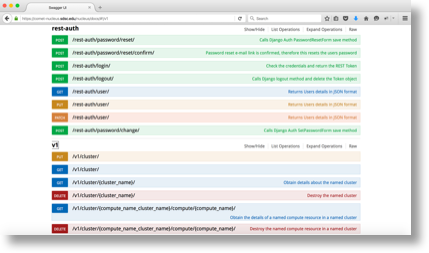
\includegraphics[width=1.0\columnwidth]{images/client/Picture1.png}
    \caption{Rest Interface}
    \label{F:1}
%\end{figure}

%\begin{figure}[htb]
  \centering
    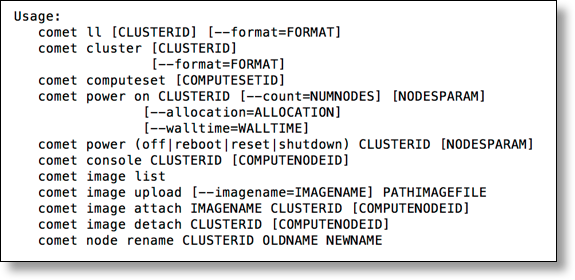
\includegraphics[width=1.0\columnwidth]{images/client/Picture2.png}
    \caption{Commandline }
    \label{F:2}
%\end{figure}

%\begin{figure}[htb]
  \centering
    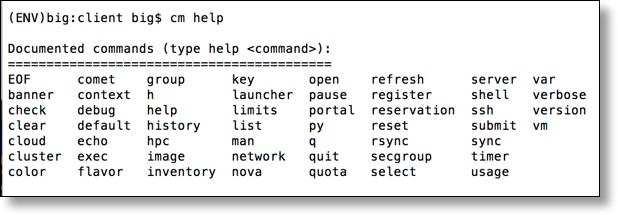
\includegraphics[width=1.0\columnwidth]{images/client/Picture3.png}
    \caption{Command Shell}
    \label{F:3}
%\end{figure}
\end{comment}






\begin{comment}
\begin{figure}[htb]
  \centering
    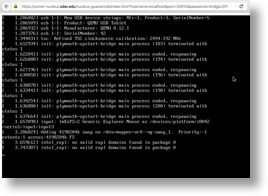
\includegraphics[width=1.0\columnwidth]{images/client/Picture4.png}
    \caption{4}
    \label{F:4}
\end{figure}
\end{comment}

\begin{comment}
%\begin{figure}[htb]
  \centering
    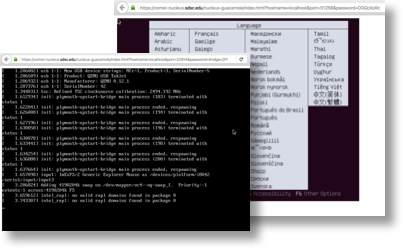
\includegraphics[width=1.0\columnwidth]{images/client/Picture5.png}
    \caption{Console}
    \label{F:5}
\end{figure}
\end{comment}
